\documentclass[../main.tex]{subfiles}

\begin{document}

\section{e-Game Rules}

\subsection{Objective}

Be the last surviving meeple on the board.

\subsection{Players}

Each team consists of two people:
\begin{itemize}
    \item \textbf{Mover (Pawn Controller)}: Controls the movement of the meeple on the board.
    \item \textbf{Operator (Strategist)}: Makes decisions on whether to shoot or pass the bullet without seeing the board.
\end{itemize}

\subsection{Game Components}
\begin{itemize}
    \item \textbf{Magnetic board(s)}: Includes hidden magnets under each position.
    \item \textbf{Meeples (pawns)}: Each player team has one meeple. It has two LEDs: one for knowing who has the bullet and another for magnet detection feedback.
    \item \textbf{Operation Base}: Includes LCD display, push button, and other components for decisions made by operators.
    \item \textbf{Broker}: Handles the game logic and the state.
\end{itemize}

\subsection{Setup}
\begin{itemize}
    \item \textbf{Initial Meeple Placement}: Each pawn begins in a random position on the board. This is decided before the game starts.
    \item \textbf{Bullet Assignment}: One player is randomly assigned the Bullet at the start of the game.
\end{itemize}

\subsection{Gameplay Overview}
The game proceeds in rounds, with the following steps repeated until only one meeple remains:
\begin{enumerate}
    \item \textbf{Movement Phase:}
    \begin{itemize}
        \item Pawns move one space in one of four directions: up, down, left, or right.
        \item Movement order is decided randomly at the start of each round.
    \end{itemize}
    \item \textbf{Decision Phase:}
    \begin{itemize}
        \item The operator of the team with the Bullet decides if they want to shoot.
        \item The operator cannot see the board, but may communicate with other pawns (within 60 seconds).
        \item Shooting affects all meeples in the same row, column, or diagonal as the operator's meeple (Figure \ref{fig:shooting}).
        \begin{itemize}
            \item \textbf{Hit}: If the shot hits any meeples, they are eliminated.
            \item \textbf{Miss}: If no other meeple is hit, the shooting operator is eliminated.
        \end{itemize}
        \item If the operator chooses not to shoot, there is a small probability of dying.
    \end{itemize}
\end{enumerate}

\begin{figure}[!htb]
    \centering
    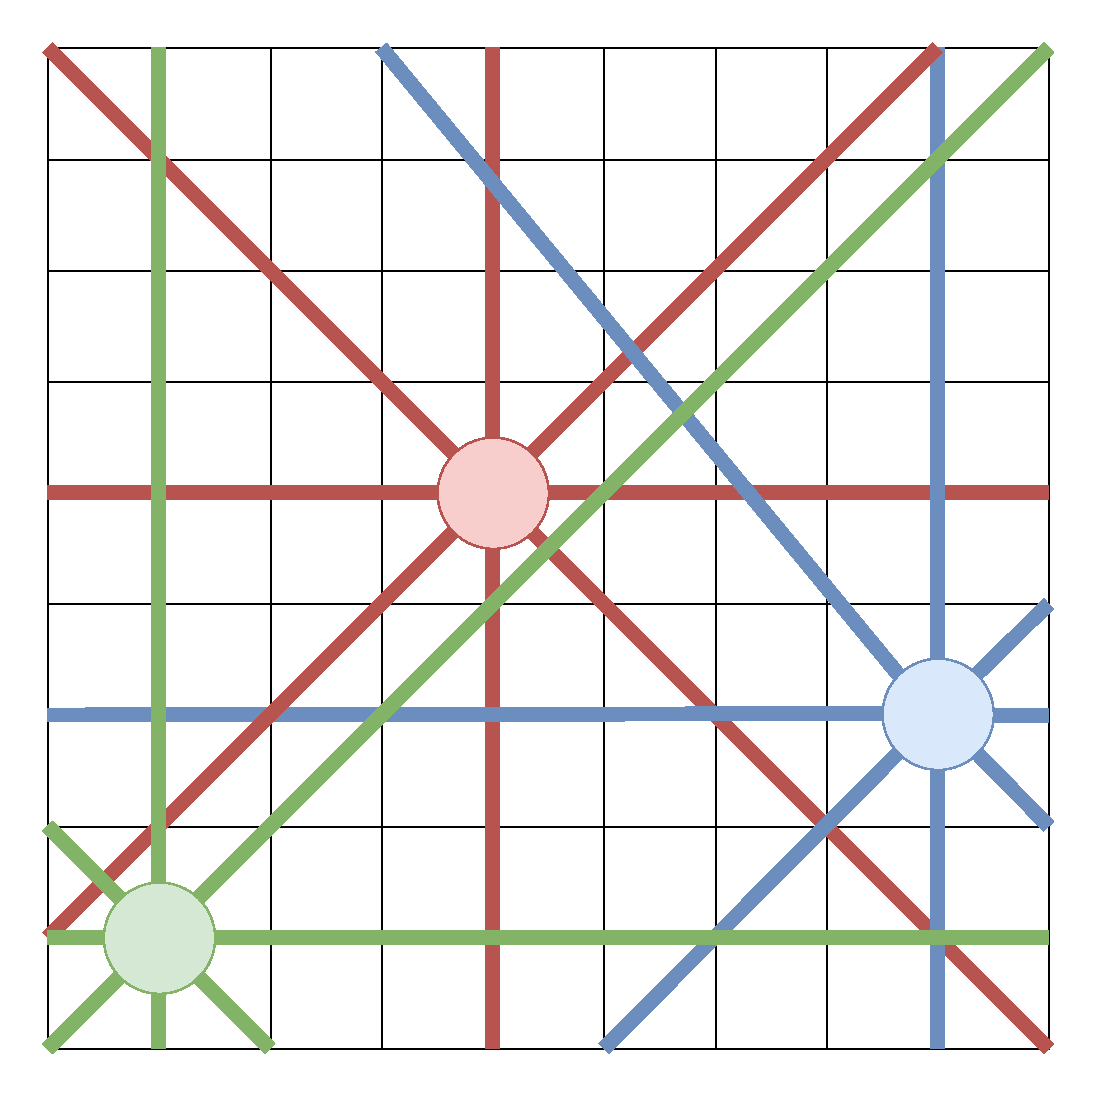
\includegraphics[width= 0.5\linewidth]{\subfix{../media/figures/shooting.pdf}}\
    \caption{Shooting directions examples}
    \label{fig:shooting}
\end{figure}

\subsection{Additional Rules}
\begin{itemize}
    \item \textbf{Time Constraints}: Operators must decide to shoot or not within 60 seconds. If time runs out, the decision is to not shoot.
    \item \textbf{Lives}: Each meeple has 1 life. If they are hit, they are eliminated.
    \item \textbf{Random Player Selection}: When the bullet is reassigned, the game selects a random player who hasn’t been eliminated.
\end{itemize}

\subsection{End Condition}
The game continues until only one meeple remains. This team is declared the winner.

\end{document}
